\documentclass[10pt]{article}

\input{../preambule}
\input{../styles}
\input{../bas_de_page_quatrieme} 
 
%%%%%%%%%%%   Marges de pages  %%%%%%%%%%%%%%%% 
 \usepackage{geometry}
 \geometry{top=1cm, bottom=0cm, left=2cm , right=2cm}
%%%%%%%%%%%%%%%%%%%%%%%%%%%%%%%%%%%%%%%%%%%%%%%

%%%%%%%%%%%%%%%  Indentation  %%%%%%%%%%%%%%%%%%
\parindent=0pt
%%%%%%%%%%%%%%%%%%%%%%%%%%%%%%%%%%%%%%%%%%%%%%%%


\begin{document}

%%%%%%%%%%%%%%%%%%%%%%%%%%%%%%%%%%%%%%%%%%%%%%%
%%%%		 Titre encadré
%%%%%%%%%%%%%%%%%%%%%%%%%%%%%%%%%%%%%%%%%%%%%%%
\begin{encadrementombre} {Thème 10 Statistiques}
{\LARGE DTL17: Statistiques; pourcentages}\\

%% Laisse la ligne vide ci-dessus
{\Large Gestion de données}
\end{encadrementombre}


%%%%%%%%%%%%%%%%%%%%%%%%%%%%%%%%%%%%%%%%%%%%%%%
%%%%		 Corps du document
%%%%%%%%%%%%%%%%%%%%%%%%%%%%%%%%%%%%%%%%%%%%%%%

%%%%%%%%%%%%%%%%%%%%%%%%%%%%%%%%%%%%%%%%%%%%%%%
%%%% \renewcommand{\arraystretch}{1.8}
\definecolor{shadecolor}{gray}{0.9}
%%%%%%%%%%%%%%%%%%%%%%%%%%%%%%%%%%%%%%%%%%%%%%%
%%%%%%%%%%%   Hauteur de ligne  %%%%%%%%%%%%%%%%
{\setlength{\baselineskip}{1.5\baselineskip}
%%%%%%%%%%%%%%%%%%%%%%%%%%%%%%%%%%%%%%%%%%%%%%%%


\begin{exo} \textbf{1}(voir sesamath)\\
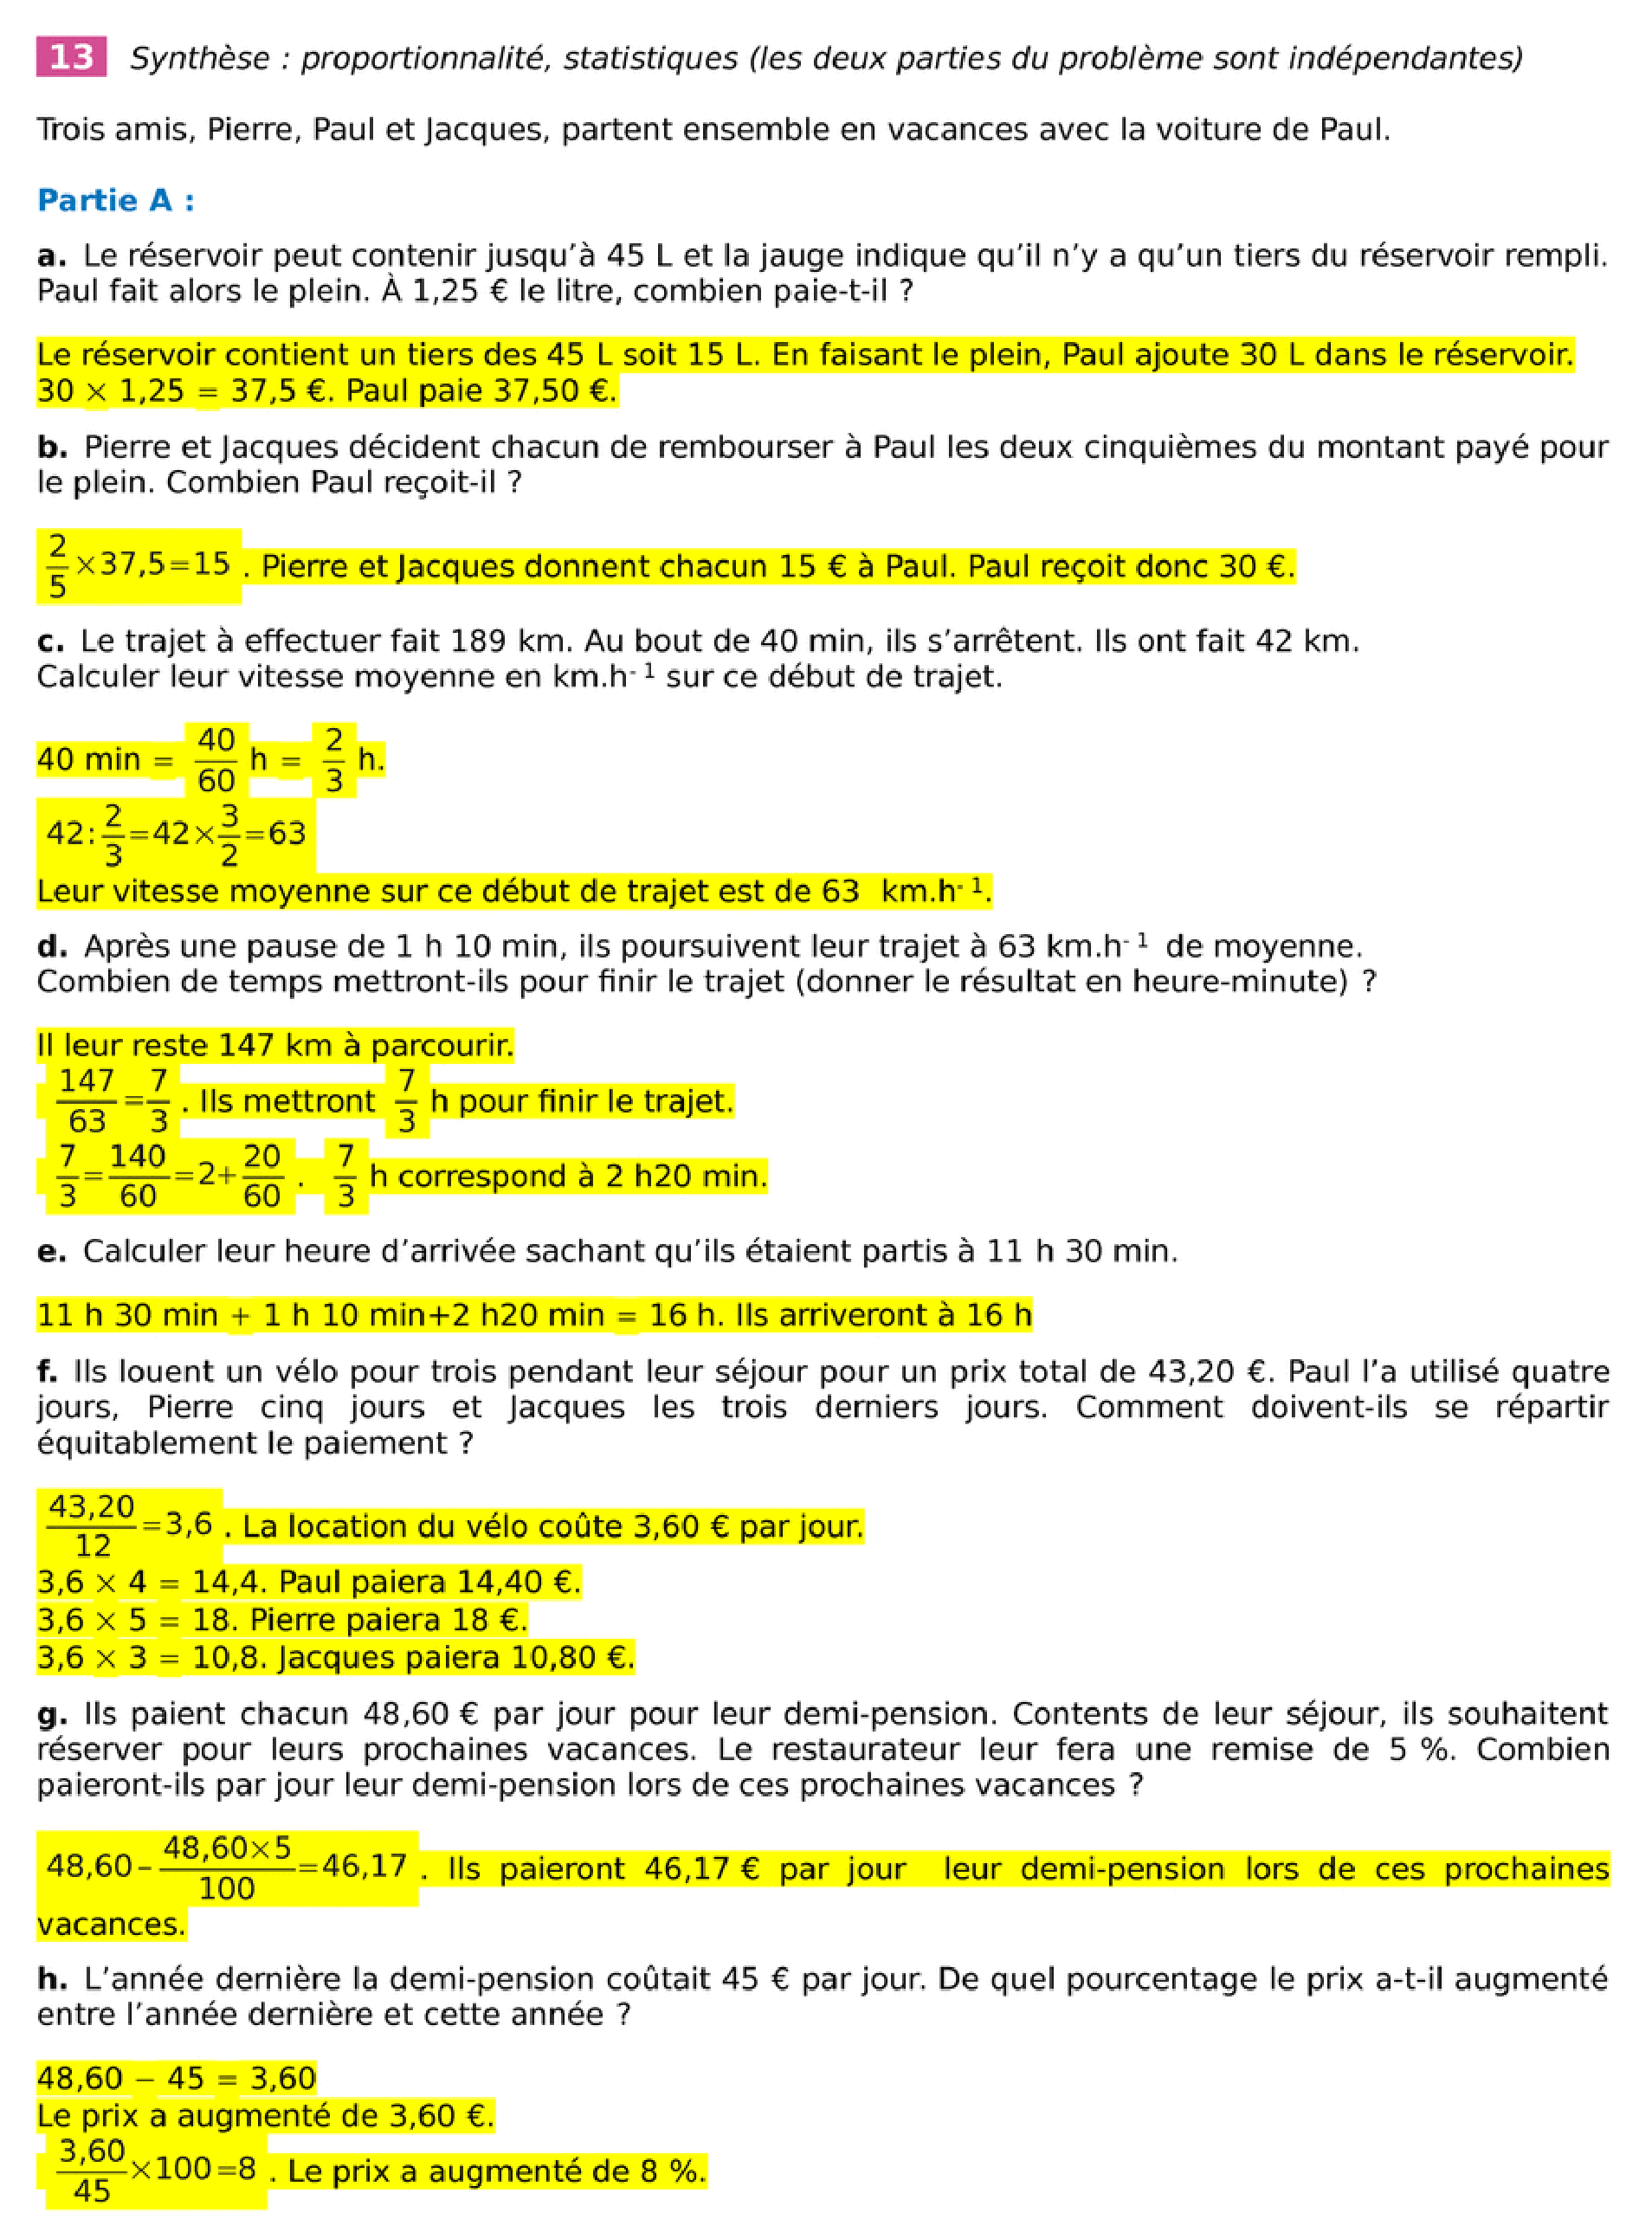
\includegraphics[scale=0.5]{DTL17_statistiques_pourcentages_cor.eps}\\
 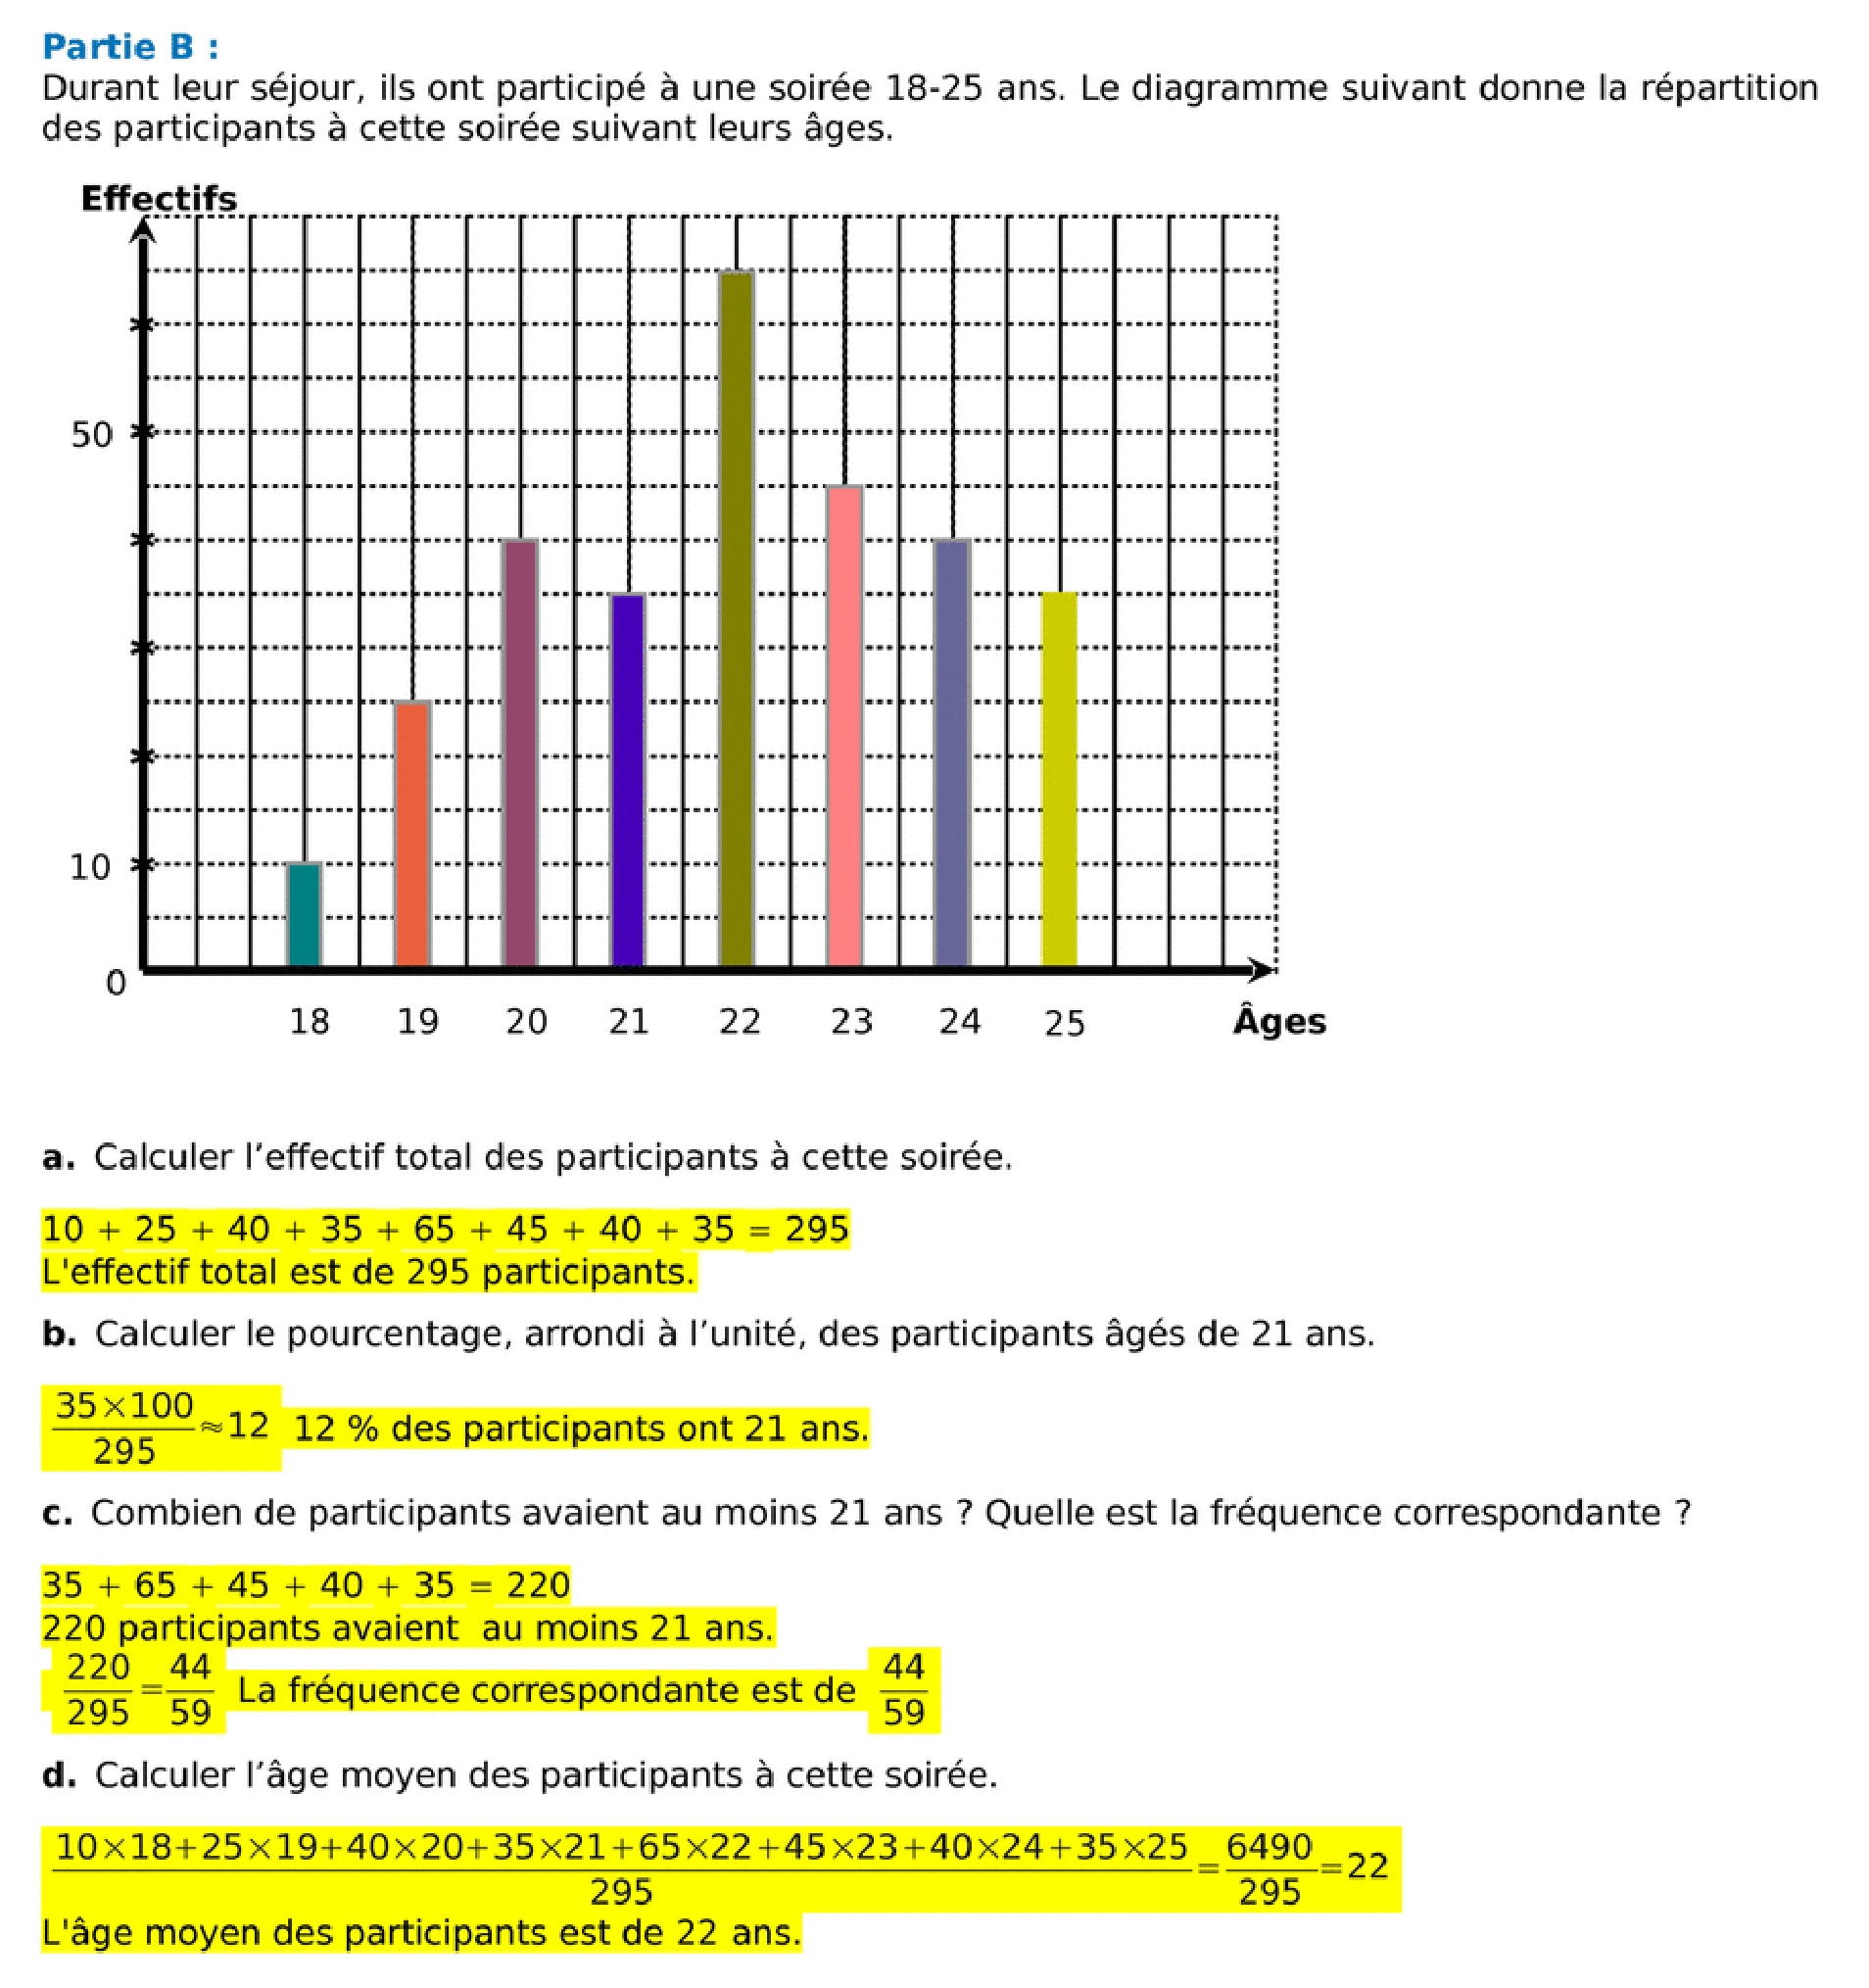
\includegraphics[scale=0.5]{DTL17_statistiques_pourcentages2_cor.eps}
\end{exo}






\end{document}